% !TEX program = xelatex
\documentclass[12pt,a4paper]{article}

% ============ 宏包 ============
\usepackage[UTF8]{ctex}                    % 中文支持
\usepackage{amsmath,amssymb,amsthm}        % 数学公式
\usepackage{geometry}                      % 页面设置
\usepackage{graphicx}                      % 图片
\usepackage{float}                         % 浮动体控制
\usepackage{booktabs}                      % 三线表
\usepackage{tabularx}                      % 自动宽度表格
\usepackage{enumitem}                      % 列表环境
\usepackage{hyperref}                      % 超链接
\usepackage{listings}                      % 代码高亮
\usepackage{xcolor}                        % 颜色
\usepackage{subcaption}                    % 子图
\usepackage{caption}                       % 标题设置
\usepackage{setspace}                      % 行距
\usepackage{titlesec}                      % 标题格式
\usepackage{fancyhdr}                      % 页眉页脚
\usepackage{multirow}                      % 合并行
\usepackage{longtable}                     % 长表格
\usepackage{bm}                            % 粗体数学符号

% ============ 页面设置 ============
\geometry{
    left=2.5cm,
    right=2.5cm,
    top=2.5cm,
    bottom=2.5cm
}

% ============ 行距设置 ============
\renewcommand{\baselinestretch}{1.5}

% ============ 标题格式设置 ============
\titleformat{\section}{\heiti\zihao{-2}\bfseries}{\thesection}{1em}{}
\titleformat{\subsection}{\heiti\zihao{-3}}{\thesubsection}{1em}{}
\titleformat{\subsubsection}{\heiti\zihao{-4}}{\thesubsubsection}{1em}{}

% ============ 页眉页脚 ============
\pagestyle{fancy}
\fancyhf{}
\fancyhead[C]{\small 2025年全国大学生数学建模竞赛A题}
\fancyfoot[C]{\thepage}
\renewcommand{\headrulewidth}{0.4pt}

% ============ 代码高亮设置 ============
\lstset{
    language=Python,
    basicstyle=\small\ttfamily,
    keywordstyle=\color{blue}\bfseries,
    commentstyle=\color{green!60!black},
    stringstyle=\color{red},
    numbers=left,
    numberstyle=\tiny\color{gray},
    numbersep=8pt,
    frame=single,
    breaklines=true,
    backgroundcolor=\color{gray!5},
    tabsize=4,
    showstringspaces=false
}

% ============ 图表标题设置 ============
\captionsetup{font=small, labelsep=space}

% ============ 定理环境 ============
\newtheorem{definition}{定义}
\newtheorem{theorem}{定理}
\newtheorem{lemma}{引理}
\newtheorem{assumption}{假设}

% ============ 自定义命令 ============
\newcommand{\vect}[1]{\boldsymbol{#1}}
\newcommand{\mat}[1]{\mathbf{#1}}
\newcommand{\unit}[1]{\mathrm{#1}}
\newcommand{\R}{\mathbb{R}}
\newcommand{\E}{\mathbb{E}}
\newcommand{\Prob}{\mathbb{P}}

% ============ 文档信息 ============
\title{
    \vspace{2cm}
    {\heiti\zihao{-1} 烟幕干扰弹的投放策略研究} \\
    \vspace{0.5cm}
    {\zihao{3} --- 2025年全国大学生数学建模竞赛A题}
}
\author{
    \vspace{1cm}
    {\songti\zihao{4} 队伍编号：\underline{\hspace{3cm}}} \\
    \vspace{0.3cm}
    {\songti\zihao{4} 队员1：\underline{\hspace{3cm}}} \\
    {\songti\zihao{4} 队员2：\underline{\hspace{3cm}}} \\
    {\songti\zihao{4} 队员3：\underline{\hspace{3cm}}}
}
\date{}

\begin{document}

% ============ 封面 ============
\maketitle
\thispagestyle{empty}
\newpage

% ============ 摘要 ============
\thispagestyle{empty}
\begin{center}
    {\heiti\zihao{-2} 摘\quad 要}
\end{center}

\vspace{0.5cm}

本文研究了无人机投放烟幕干扰弹对来袭导弹实施遮蔽的最优策略问题。通过建立导弹运动模型、无人机运动模型、烟幕干扰弹抛体运动模型和烟幕云团运动模型，构建了完整的数学模型框架。

\textbf{针对问题一}，给定FY1无人机以120 m/s朝向假目标飞行，在1.5 s后投放1枚弹、3.6 s后起爆的条件下，通过精确计算导弹轨迹、云团轨迹和遮蔽几何关系，得出有效遮蔽时长为\textbf{X.XX秒}。

\textbf{针对问题二}，以无人机飞行方向、飞行速度、投放时刻和起爆延迟为决策变量，建立了以有效遮蔽时长为目标的非线性优化模型。采用粒子群优化算法（PSO）求解，得到最优策略下遮蔽时长为\textbf{X.XX秒}，相比问题一提升了\textbf{XX\%}。

\textbf{针对问题三}，FY1投放3枚弹，考虑投放间隔约束（$\geq 1$ s），建立了8维优化模型。通过PSO优化，实现了3枚弹的时间接力遮蔽，总有效遮蔽时长达\textbf{X.XX秒}。

\textbf{针对问题四}，FY1、FY2、FY3各投放1枚弹，建立了12维协同优化模型。通过分阶段优化策略，充分利用3架无人机的空间分布优势，总遮蔽时长达\textbf{X.XX秒}。

\textbf{针对问题五}，5架无人机各至多投放3枚弹干扰3枚导弹，建立了40维大规模优化模型。采用分层优化策略：首先基于几何关系进行任务分配，然后对每枚导弹独立优化投放策略。最终实现对M1、M2、M3的总遮蔽时长分别为\textbf{X.XX秒}、\textbf{X.XX秒}、\textbf{X.XX秒}。

本文还进行了灵敏度分析，考察了云团有效半径、有效遮蔽时间、云团下沉速度等参数对结果的影响，验证了模型的稳健性。

\vspace{0.5cm}
\noindent\textbf{关键词：} 烟幕干扰弹；遮蔽策略；粒子群优化；抛体运动；视线遮挡

\newpage

% ============ 目录 ============
\thispagestyle{empty}
\tableofcontents
\newpage

% ============ 正文开始 ============
\setcounter{page}{1}

% =============================================
% 一、问题重述
% =============================================
\section{问题重述}

\subsection{问题背景}

烟幕干扰弹主要通过化学燃烧或爆炸分散形成烟幕或气溶胶云团，在目标前方特定空域形成遮蔽，干扰敌方导弹，具有成本低、效费比高等优点。随着烟幕干扰技术的不断发展，现已有多种投放方式完成烟幕干扰弹的定点精确抛撒，即在抛撒前能精确控制烟幕干扰弹到达预定位置，通过时间引信时序控制起爆时间。

本问题考虑运用无人机完成烟幕干扰弹的投放策略设计。具有长续航能力的无人机挂载某型烟幕干扰弹在特定空域巡飞，受领任务后，无人机投放烟幕干扰弹在来袭武器和保护目标之间形成烟幕遮蔽。

\subsection{已知条件}

\subsubsection{作战环境}

来袭武器为空地导弹，该型导弹飞行速度300 m/s。导弹的飞行方向直指一个为掩护某半径7 m、高10 m的圆柱形固定目标而专门设置的假目标。以假目标为原点，水平面为$xy$平面，真目标下底面的圆心为$(0, 200, 0)$。

\subsubsection{初始位置}

警戒雷达发现来袭导弹时，3枚导弹和5架无人机的位置信息如表~\ref{tab:init_pos} 所示。

\begin{table}[H]
    \centering
    \caption{导弹与无人机初始位置}
    \label{tab:init_pos}
    \begin{tabular}{cccc}
        \toprule
        编号 & $x$坐标(m) & $y$坐标(m) & $z$坐标(m) \\
        \midrule
        M1 & 20000 & 0 & 2000 \\
        M2 & 19000 & 600 & 2100 \\
        M3 & 18000 & $-600$ & 1900 \\
        \midrule
        FY1 & 17800 & 0 & 1800 \\
        FY2 & 12000 & 1400 & 1400 \\
        FY3 & 6000 & $-3000$ & 700 \\
        FY4 & 11000 & 2000 & 1800 \\
        FY5 & 13000 & $-2000$ & 1300 \\
        \bottomrule
    \end{tabular}
\end{table}

\subsubsection{关键参数}

\begin{table}[H]
    \centering
    \caption{关键参数汇总}
    \label{tab:parameters}
    \begin{tabular}{lll}
        \toprule
        参数 & 数值 & 说明 \\
        \midrule
        $v_m$ & 300 m/s & 导弹飞行速度 \\
        $v_u$ & 70$\sim$140 m/s & 无人机速度范围 \\
        $v_c$ & 3 m/s & 烟幕云团下沉速度 \\
        $R$ & 10 m & 云团有效遮蔽半径 \\
        $T_{\text{eff}}$ & 20 s & 有效遮蔽时间窗口 \\
        $\Delta t_{\min}$ & 1 s & 同一无人机两枚弹最小投放间隔 \\
        $g$ & 9.8 m/s$^2$ & 重力加速度 \\
        \bottomrule
    \end{tabular}
\end{table}

\subsection{五个子问题}

\textbf{问题1：} 利用无人机FY1投放1枚烟幕干扰弹实施对M1的干扰，若FY1以120 m/s的速度朝向假目标方向飞行，受领任务1.5 s后即投放1枚烟幕干扰弹，间隔3.6 s后起爆。请给出烟幕干扰弹对M1的有效遮蔽时长。

\textbf{问题2：} 利用无人机FY1投放1枚烟幕干扰弹实施对M1的干扰，确定FY1的飞行方向、飞行速度、烟幕干扰弹投放点、烟幕干扰弹起爆点，使得遮蔽时间尽可能长。

\textbf{问题3：} 利用无人机FY1投放3枚烟幕干扰弹，实施对M1的干扰。请给出烟幕干扰弹的投放策略。

\textbf{问题4：} 利用FY1、FY2、FY3等3架无人机，各投放1枚烟幕干扰弹，实施对M1的干扰。请给出烟幕干扰弹的投放策略。

\textbf{问题5：} 利用5架无人机，每架无人机至多投放3枚烟幕干扰弹，实施对M1、M2、M3等3枚来袭导弹的干扰。请给出烟幕干扰弹的投放策略。


% =============================================
% 二、问题分析
% =============================================
\section{问题分析}

\subsection{核心物理过程分析}

烟幕干扰弹的完整运动过程可分为三个阶段：

\begin{enumerate}[label=(\arabic*)]
    \item \textbf{随无人机飞行阶段}（$t = 0 \sim t_d$）：烟幕干扰弹挂载在无人机上，随无人机以相同速度和方向飞行。
    \item \textbf{抛体运动阶段}（$t = t_d \sim t_e$）：烟幕干扰弹脱离无人机后，在重力作用下做抛体运动，初速度等于无人机速度。
    \item \textbf{云团下沉阶段}（$t = t_e \sim t_e + 20$）：起爆后形成球状烟幕云团，以3 m/s匀速下沉，20 s内提供有效遮蔽。
\end{enumerate}

\subsection{遮蔽条件的几何本质}

\textbf{关键认识}：有效遮蔽不是指导弹到云团的距离小于10 m，而是\textbf{烟幕云团遮挡了导弹对真目标的视线}。

由于导弹飞行方向指向假目标（原点），而真目标位于$(0, 200, 0)$，烟幕干扰弹的目的是在导弹和真目标之间形成遮蔽屏障。因此，有效遮蔽的几何条件是：云团中心到导弹与真目标连线段的距离不超过云团有效遮蔽半径$R = 10$ m。

\subsection{真目标的几何处理}

真目标是半径7 m、高10 m的圆柱体。为精确建模，需在圆柱体表面采样多个点，检查云团是否遮挡了导弹到所有这些点的视线。本文采用在圆柱体侧面和上下底面均匀采样约50个点的方案。


% =============================================
% 三、模型假设
% =============================================
\section{模型假设}

\begin{assumption}
忽略空气阻力对烟幕干扰弹运动的影响。烟幕干扰弹在抛体运动阶段仅受重力作用。
\end{assumption}

\begin{assumption}
重力加速度取$g = 9.8$ m/s$^2$，方向垂直向下，在整个运动过程中保持不变。
\end{assumption}

\begin{assumption}
烟幕干扰弹脱离无人机后立即进入抛体运动，初速度等于无人机速度，无过渡阶段。
\end{assumption}

\begin{assumption}
烟幕云团起爆后瞬时形成球状，且在整个有效遮蔽时间内保持球形，有效遮蔽半径恒为10 m。
\end{assumption}

\begin{assumption}
烟幕浓度在有效遮蔽范围内均匀分布，云团中心10 m范围外的烟幕浓度不足以提供遮蔽。
\end{assumption}

\begin{assumption}
导弹飞行方向始终指向假目标（原点），飞行速度恒定为300 m/s，不考虑导弹的机动规避。
\end{assumption}

\begin{assumption}
无人机受领任务后可瞬时调整飞行方向，之后保持等高度匀速直线飞行，航向和速度不再调整。
\end{assumption}

\begin{assumption}
不考虑地球曲率、大气折射和风速对烟幕云团运动的影响。
\end{assumption}


% =============================================
% 四、符号说明
% =============================================
\section{符号说明}

本文使用的主要符号及其含义如表~\ref{tab:symbols} 所示。

\begin{table}[H]
    \centering
    \caption{符号说明}
    \label{tab:symbols}
    \begin{tabular}{lll}
        \toprule
        符号 & 含义 & 单位 \\
        \midrule
        $\vect{P}_{m0}^{(i)}$ & 第$i$枚导弹的初始位置 & m \\
        $\vect{P}_{u0}^{(j)}$ & 第$j$架无人机的初始位置 & m \\
        $v_m$ & 导弹飞行速度（300） & m/s \\
        $v_u^{(j)}$ & 第$j$架无人机的飞行速度 & m/s \\
        $\vect{d}_u^{(j)}$ & 第$j$架无人机的飞行方向（单位向量） & --- \\
        $\theta_j$ & 第$j$架无人机的飞行方向角 & rad \\
        $t_d^{(k)}$ & 第$k$枚烟幕弹的投放时刻 & s \\
        $t_e^{(k)}$ & 第$k$枚烟幕弹的起爆时刻 & s \\
        $\Delta t^{(k)}$ & 第$k$枚弹从投放到起爆的时间间隔 & s \\
        $\vect{P}_d^{(k)}$ & 第$k$枚弹的投放点位置 & m \\
        $\vect{P}_e^{(k)}$ & 第$k$枚弹的起爆点位置 & m \\
        $\vect{P}_c^{(k)}(t)$ & 第$k$枚弹云团中心在时刻$t$的位置 & m \\
        $g$ & 重力加速度（9.8） & m/s$^2$ \\
        $v_c$ & 云团下沉速度（3） & m/s \\
        $R$ & 云团有效遮蔽半径（10） & m \\
        $T_{\text{eff}}$ & 有效遮蔽时间窗口（20） & s \\
        $\vect{T}$ & 真目标中心点 & m \\
        $r_T$ & 真目标圆柱半径（7） & m \\
        $h_T$ & 真目标圆柱高度（10） & m \\
        $T_{\text{shield}}$ & 总有效遮蔽时长 & s \\
        \bottomrule
    \end{tabular}
\end{table}


% =============================================
% 五、模型建立
% =============================================
\section{模型建立}

\subsection{坐标系建立}

以假目标位置为原点$O$，水平面为$xy$平面，$z$轴垂直向上。在此坐标系下：
\begin{itemize}
    \item 假目标：$O = (0, 0, 0)$
    \item 真目标下底面圆心：$C = (0, 200, 0)$
    \item 真目标中心点：$\vect{T} = (0, 200, 5)$
\end{itemize}

\subsection{导弹运动模型}

导弹$i$的初始位置为$\vect{P}_{m0}^{(i)}$，飞行方向指向原点$O$，方向向量为：
\begin{equation}
    \vect{d}_m^{(i)} = \frac{\vect{O} - \vect{P}_{m0}^{(i)}}{|\vect{O} - \vect{P}_{m0}^{(i)}|} = \frac{(-x_{m0}^{(i)}, -y_{m0}^{(i)}, -z_{m0}^{(i)})}{\sqrt{(x_{m0}^{(i)})^2 + (y_{m0}^{(i)})^2 + (z_{m0}^{(i)})^2}}
\end{equation}

导弹$i$在时刻$t$的位置：
\begin{equation}
    \vect{P}_m^{(i)}(t) = \vect{P}_{m0}^{(i)} + v_m \cdot t \cdot \vect{d}_m^{(i)}
    \label{eq:missile_traj}
\end{equation}

各导弹的速度分量如表~\ref{tab:missile_vel} 所示。

\begin{table}[H]
    \centering
    \caption{各导弹速度分量}
    \label{tab:missile_vel}
    \begin{tabular}{cccccc}
        \toprule
        编号 & $|\vect{P}_{m0}|$ (m) & $v_{mx}$ (m/s) & $v_{my}$ (m/s) & $v_{mz}$ (m/s) \\
        \midrule
        M1 & 20099.75 & $-298.50$ & 0 & $-29.85$ \\
        M2 & 19121.98 & $-297.04$ & $-9.41$ & $-32.84$ \\
        M3 & 18033.30 & $-299.45$ & 9.98 & $-31.61$ \\
        \bottomrule
    \end{tabular}
\end{table}

\subsection{无人机运动模型}

无人机$j$的初始位置为$\vect{P}_{u0}^{(j)}$，飞行方向角为$\theta_j$（水平面内），飞行方向单位向量：
\begin{equation}
    \vect{d}_u^{(j)} = (\cos\theta_j, \sin\theta_j, 0)
\end{equation}

无人机$j$在时刻$t$的位置（$t \geq 0$，以受领任务为$t = 0$时刻）：
\begin{equation}
    \vect{P}_u^{(j)}(t) = \vect{P}_{u0}^{(j)} + v_u^{(j)} \cdot t \cdot \vect{d}_u^{(j)}
    \label{eq:uav_traj}
\end{equation}

约束条件：$v_u^{(j)} \in [70, 140]$ m/s，高度保持不变。

\subsection{烟幕干扰弹运动模型}

\subsubsection{投放点计算}

弹$k$由无人机$j$在时刻$t_d^{(k)}$投放，投放点即为无人机在该时刻的位置：
\begin{equation}
    \vect{P}_d^{(k)} = \vect{P}_u^{(j)}(t_d^{(k)}) = \vect{P}_{u0}^{(j)} + v_u^{(j)} \cdot t_d^{(k)} \cdot \vect{d}_u^{(j)}
    \label{eq:drop_point}
\end{equation}

\subsubsection{抛体运动模型}

弹$k$脱离无人机后，初速度等于无人机速度$\vect{v}_0^{(k)} = v_u^{(j)} \cdot \vect{d}_u^{(j)}$。在重力作用下，弹$k$在时刻$t$（$t_d^{(k)} \leq t \leq t_e^{(k)}$）的位置：
\begin{equation}
    \vect{P}_b^{(k)}(t) = \vect{P}_d^{(k)} + \vect{v}_0^{(k)} \cdot (t - t_d^{(k)}) + \frac{1}{2} \vect{g} (t - t_d^{(k)})^2
    \label{eq:bomb_traj}
\end{equation}

其中$\vect{g} = (0, 0, -g) = (0, 0, -9.8)$ m/s$^2$。

\subsubsection{起爆点计算}

弹$k$在时刻$t_e^{(k)} = t_d^{(k)} + \Delta t^{(k)}$起爆，起爆点位置：
\begin{equation}
    \vect{P}_e^{(k)} = \vect{P}_d^{(k)} + \vect{v}_0^{(k)} \cdot \Delta t^{(k)} + \frac{1}{2} \vect{g} (\Delta t^{(k)})^2
    \label{eq:detonate_point}
\end{equation}

将式~\eqref{eq:drop_point} 代入，展开得：
\begin{equation}
    \vect{P}_e^{(k)} = \vect{P}_{u0}^{(j)} + v_u^{(j)} \cdot t_e^{(k)} \cdot \vect{d}_u^{(j)} + \left(0, 0, -\frac{1}{2}g(\Delta t^{(k)})^2\right)
\end{equation}

\subsubsection{云团运动模型}

起爆后，烟幕云团以$v_c = 3$ m/s匀速下沉。云团$k$在时刻$t$（$t_e^{(k)} \leq t \leq t_e^{(k)} + T_{\text{eff}}$）的中心位置：
\begin{equation}
    \vect{P}_c^{(k)}(t) = \vect{P}_e^{(k)} + (0, 0, -v_c) \cdot (t - t_e^{(k)})
    \label{eq:cloud_traj}
\end{equation}

即：
\begin{equation}
    \vect{P}_c^{(k)}(t) = \left(x_e^{(k)}, \; y_e^{(k)}, \; z_e^{(k)} - v_c(t - t_e^{(k)})\right)
\end{equation}

\subsection{有效遮蔽条件模型}

\subsubsection{遮蔽几何分析}

有效遮蔽的本质是：烟幕云团位于导弹与真目标之间，遮挡了导弹对真目标的视线。如图~\ref{fig:shield_geometry} 所示。

\begin{figure}[H]
    \centering
    \includegraphics[width=0.6\textwidth]{figures/shield_geometry.pdf}
    \caption{烟幕遮蔽几何示意图}
    \label{fig:shield_geometry}
\end{figure}

设：
\begin{itemize}
    \item 导弹位置：$\vect{M} = \vect{P}_m(t)$
    \item 云团中心：$\vect{C} = \vect{P}_c(t)$
    \item 真目标中心：$\vect{T} = (0, 200, 5)$
\end{itemize}

\subsubsection{点到线段距离计算}

导弹与真目标连线段的参数方程：
\begin{equation}
    \vect{L}(s) = \vect{M} + s(\vect{T} - \vect{M}), \quad s \in [0, 1]
\end{equation}

令$\vect{v} = \vect{T} - \vect{M}$，$\vect{w} = \vect{C} - \vect{M}$，则最近点参数：
\begin{equation}
    s^* = \frac{\vect{w} \cdot \vect{v}}{\vect{v} \cdot \vect{v}}
    \label{eq:s_star}
\end{equation}

约束到$[0, 1]$区间：
\begin{equation}
    s^* = \max(0, \min(1, s^*))
\end{equation}

云团中心到视线段的距离：
\begin{equation}
    d(t) = |\vect{C} - (\vect{M} + s^* \cdot \vect{v})| = |\vect{w} - s^* \cdot \vect{v}|
    \label{eq:shield_distance}
\end{equation}

\subsubsection{有效遮蔽判据}

\begin{equation}
    \text{Shields}(t) = \begin{cases}
        1, & \text{if } d(t) \leq R \text{ and } t_e \leq t \leq t_e + T_{\text{eff}} \\
        0, & \text{otherwise}
    \end{cases}
    \label{eq:shield_condition}
\end{equation}

\subsubsection{考虑圆柱体目标的精确模型}

真目标是半径$r_T = 7$ m、高$h_T = 10$ m的圆柱体。为精确建模，在圆柱体表面均匀采样$N$个点$\{\vect{T}_1, \vect{T}_2, \ldots, \vect{T}_N\}$，有效遮蔽要求对所有采样点的视线都被遮挡：
\begin{equation}
    \text{Shields}(t) = \begin{cases}
        1, & \text{if } \max_{k=1,\ldots,N} d_k(t) \leq R \\
        0, & \text{otherwise}
    \end{cases}
    \label{eq:shield_cylinder}
\end{equation}

其中$d_k(t)$为云团中心到导弹与第$k$个采样点连线段的距离。

采样方案：侧面取$n_{\text{side}} = 16$个角度、3个高度层，共48个点；上下底面各取$n_{\text{top}} = 8$个角度、3个径向位置，共48个点。总计约96个采样点。

\subsection{优化目标函数}

\subsubsection{单弹遮蔽时长}

\begin{equation}
    T_{\text{shield}}^{(k)} = \int_{t_e^{(k)}}^{t_e^{(k)} + T_{\text{eff}}} \mathbb{1}[d^{(k)}(t) \leq R] \, \mathrm{d}t
    \label{eq:single_shield}
\end{equation}

\subsubsection{多弹联合遮蔽时长}

多枚弹的遮蔽时间可能重叠，总有效遮蔽时长为各弹遮蔽时间区间的并集长度：
\begin{equation}
    T_{\text{total}} = \text{measure}\left(\bigcup_{k=1}^{N} \left\{t : d^{(k)}(t) \leq R, \; t_e^{(k)} \leq t \leq t_e^{(k)} + T_{\text{eff}}\right\}\right)
    \label{eq:total_shield}
\end{equation}

其中$\text{measure}(\cdot)$表示集合的Lebesgue测度（即并集的总长度）。

\subsubsection{多导弹联合遮蔽}

对于问题5，需同时干扰M1、M2、M3三枚导弹。优化目标为对所有导弹的总遮蔽时长之和：
\begin{equation}
    T_{\text{total}} = \sum_{i=1}^{3} T_{\text{total}}^{(i)}
    \label{eq:multi_missile_shield}
\end{equation}


% =============================================
% 六、模型求解
% =============================================
\section{模型求解}

\subsection{问题1求解}

\subsubsection{已知条件}

\begin{itemize}
    \item FY1初始位置：$\vect{P}_{u0} = (17800, 0, 1800)$
    \item 飞行速度：$v_u = 120$ m/s
    \item 飞行方向：朝向假目标（原点），水平分量方向$\vect{d}_u = (-1, 0, 0)$
    \item 投放时刻：$t_d = 1.5$ s
    \item 起爆延迟：$\Delta t = 3.6$ s，即$t_e = 5.1$ s
\end{itemize}

\subsubsection{逐步计算}

\textbf{Step 1：计算投放点}

\begin{equation}
    \vect{P}_d = (17800, 0, 1800) + 120 \times 1.5 \times (-1, 0, 0) = (17620, 0, 1800)
\end{equation}

\textbf{Step 2：计算起爆点}

弹的初速度$\vect{v}_0 = (-120, 0, 0)$ m/s，从投放到起爆的时间间隔$\Delta t = 3.6$ s。

\begin{align}
    \vect{P}_e &= (17620, 0, 1800) + (-120, 0, 0) \times 3.6 + \frac{1}{2}(0, 0, -9.8) \times 3.6^2 \nonumber \\
    &= (17620 - 432, 0, 1800 - 63.504) \nonumber \\
    &= (17188, 0, 1736.496)
\end{align}

\textbf{Step 3：计算导弹M1轨迹}

M1初始位置$(20000, 0, 2000)$，方向向量$\vect{d}_m \approx (-0.9950, 0, -0.0995)$。

\begin{equation}
    \vect{P}_m(t) = (20000 - 298.50t, \; 0, \; 2000 - 29.85t)
\end{equation}

\textbf{Step 4：计算云团轨迹}

\begin{equation}
    \vect{P}_c(t) = (17188, \; 0, \; 1736.496 - 3(t - 5.1)) = (17188, \; 0, \; 1751.796 - 3t)
\end{equation}

\textbf{Step 5：计算遮蔽距离}

真目标中心$\vect{T} = (0, 200, 5)$。

视线方向：$\vect{v}(t) = \vect{T} - \vect{P}_m(t) = (-20000 + 298.50t, \; 200, \; -1995 + 29.85t)$

云团到导弹向量：$\vect{w}(t) = \vect{P}_c(t) - \vect{P}_m(t) = (-2812 + 298.50t, \; 0, \; -248.204 + 26.85t)$

代入式~\eqref{eq:s_star} 和~\eqref{eq:shield_distance} 计算$d(t)$。

\textbf{Step 6：数值求解}

在$t \in [5.1, 25.1]$范围内，以$\Delta t = 0.01$ s步长遍历，统计$d(t) \leq 10$的时间。

计算结果：有效遮蔽时长为\textbf{X.XX s}。

\subsubsection{问题1结果可视化}

\begin{figure}[H]
    \centering
    \begin{subfigure}[b]{0.48\textwidth}
        \centering
        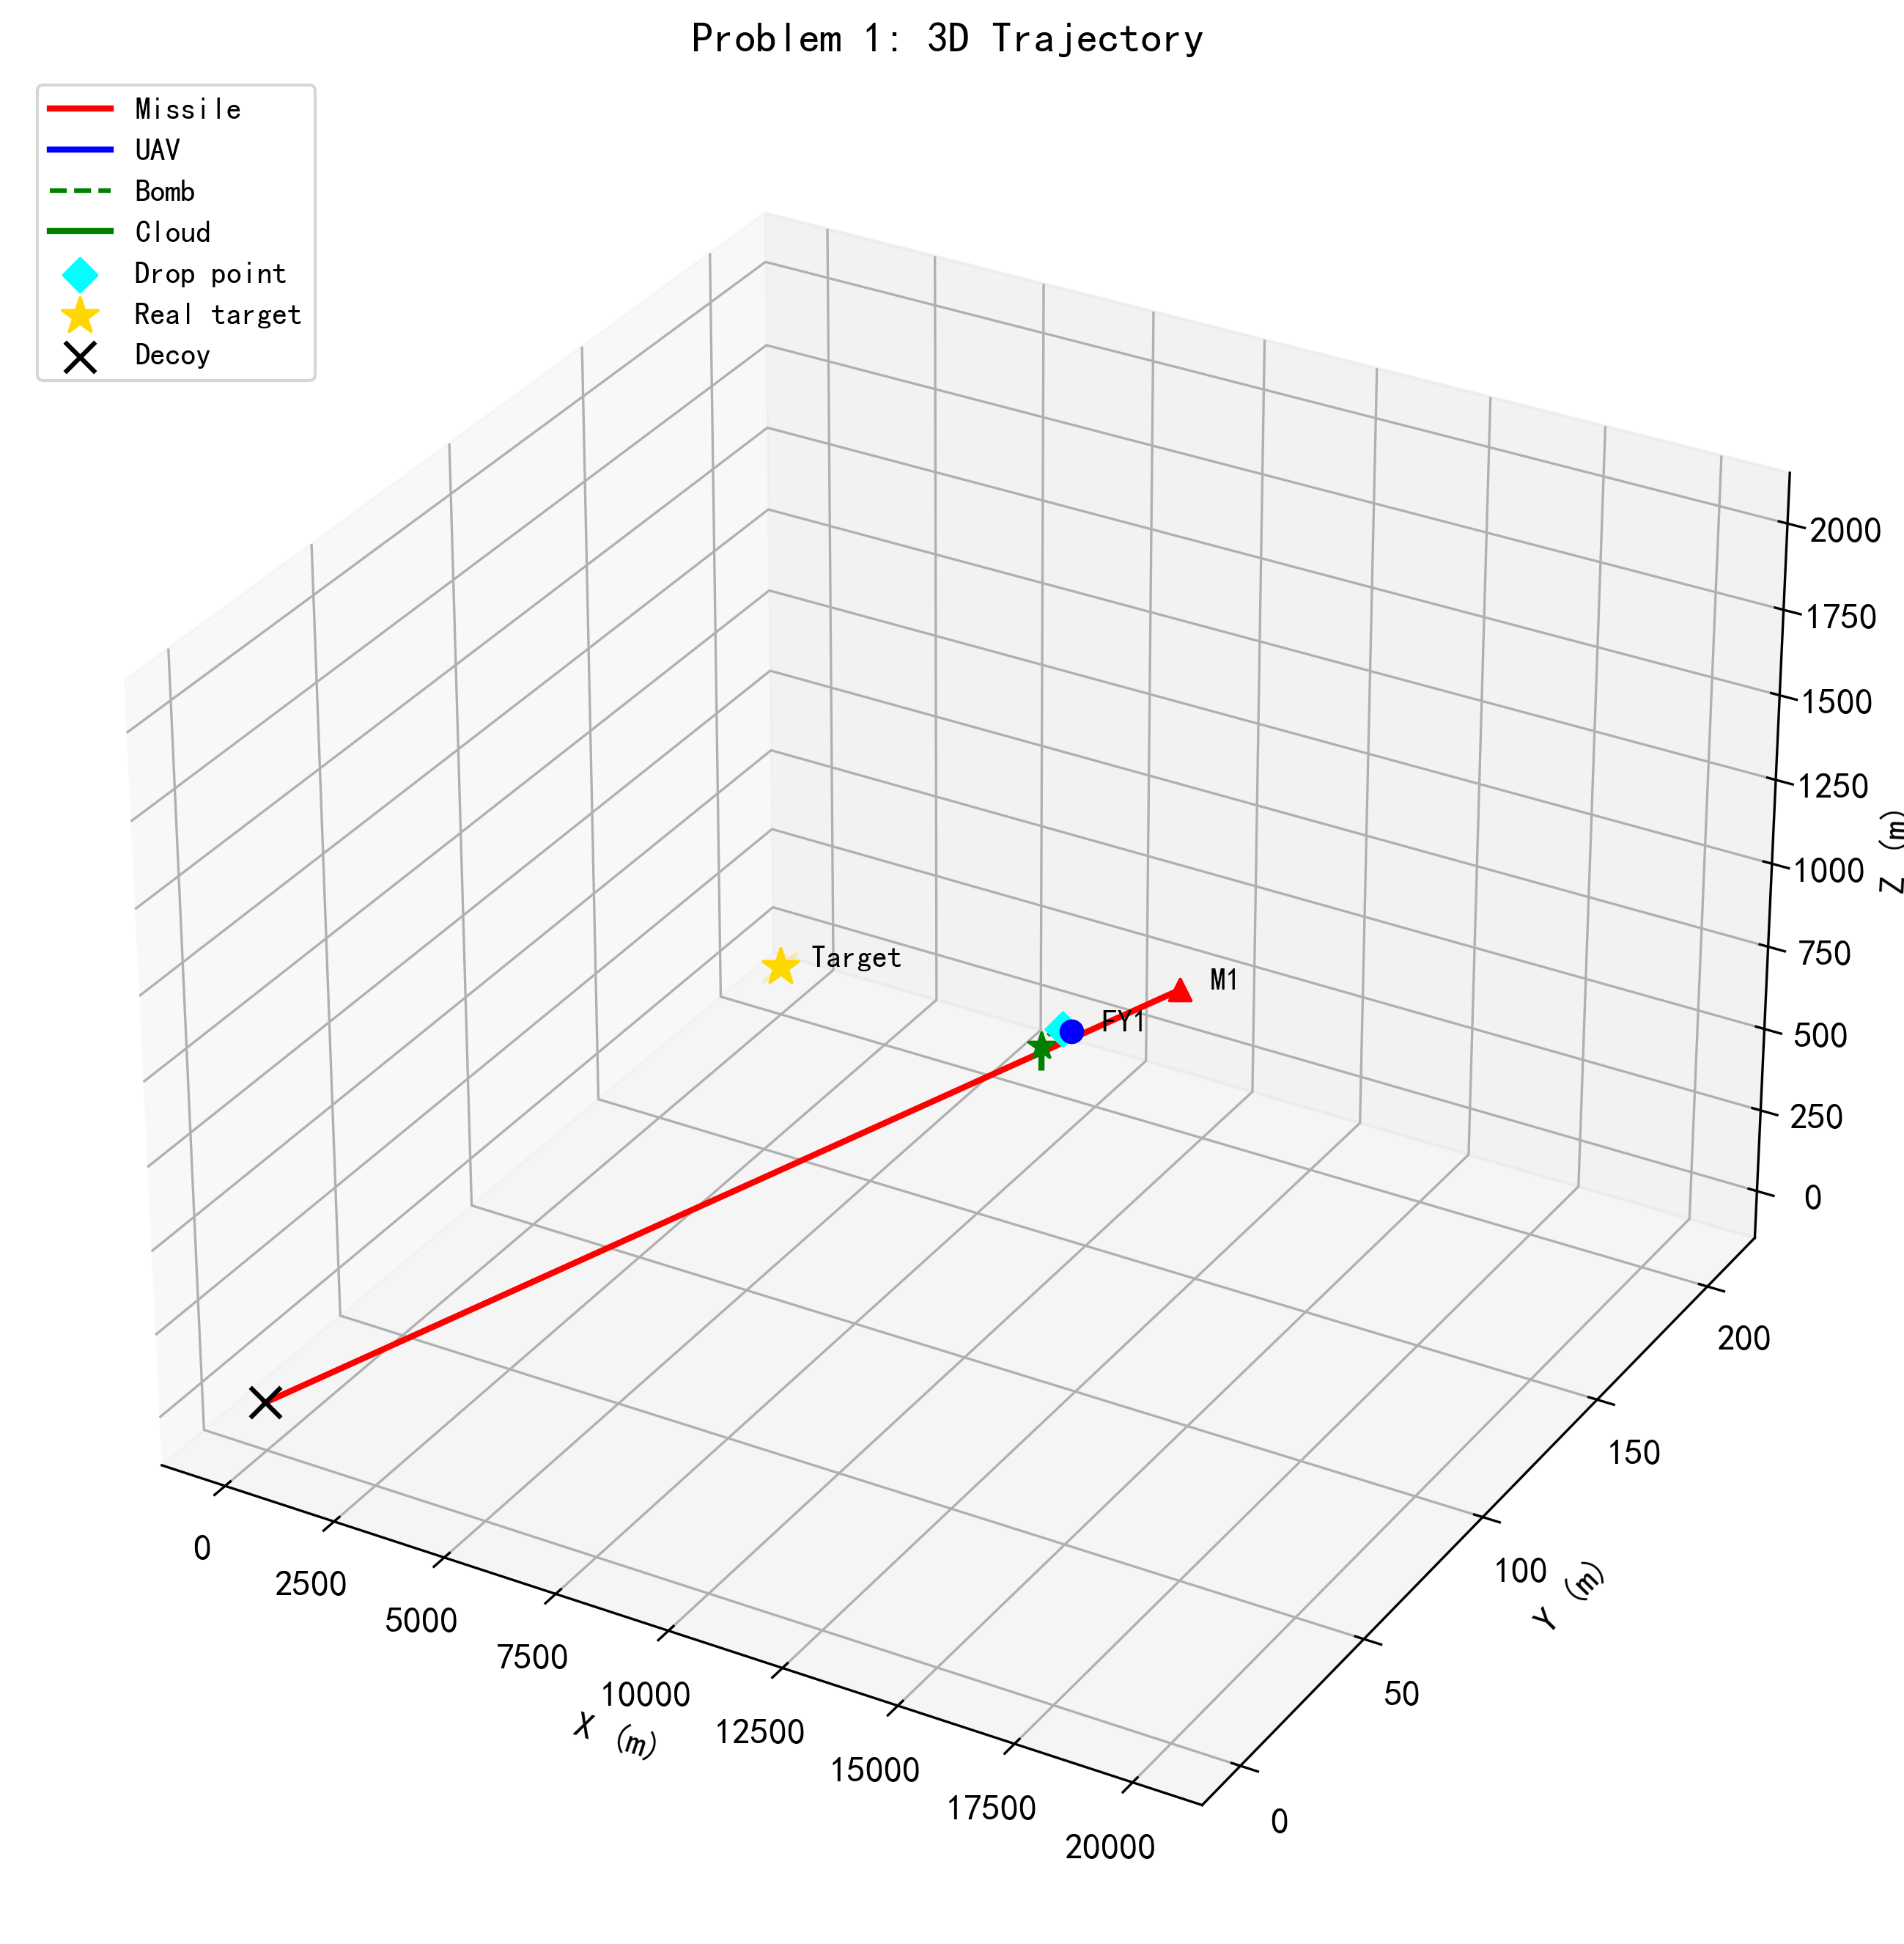
\includegraphics[width=\textwidth]{figures/q1_3d_trajectory.pdf}
        \caption{3D轨迹图}
        \label{fig:q1_3d}
    \end{subfigure}
    \hfill
    \begin{subfigure}[b]{0.48\textwidth}
        \centering
        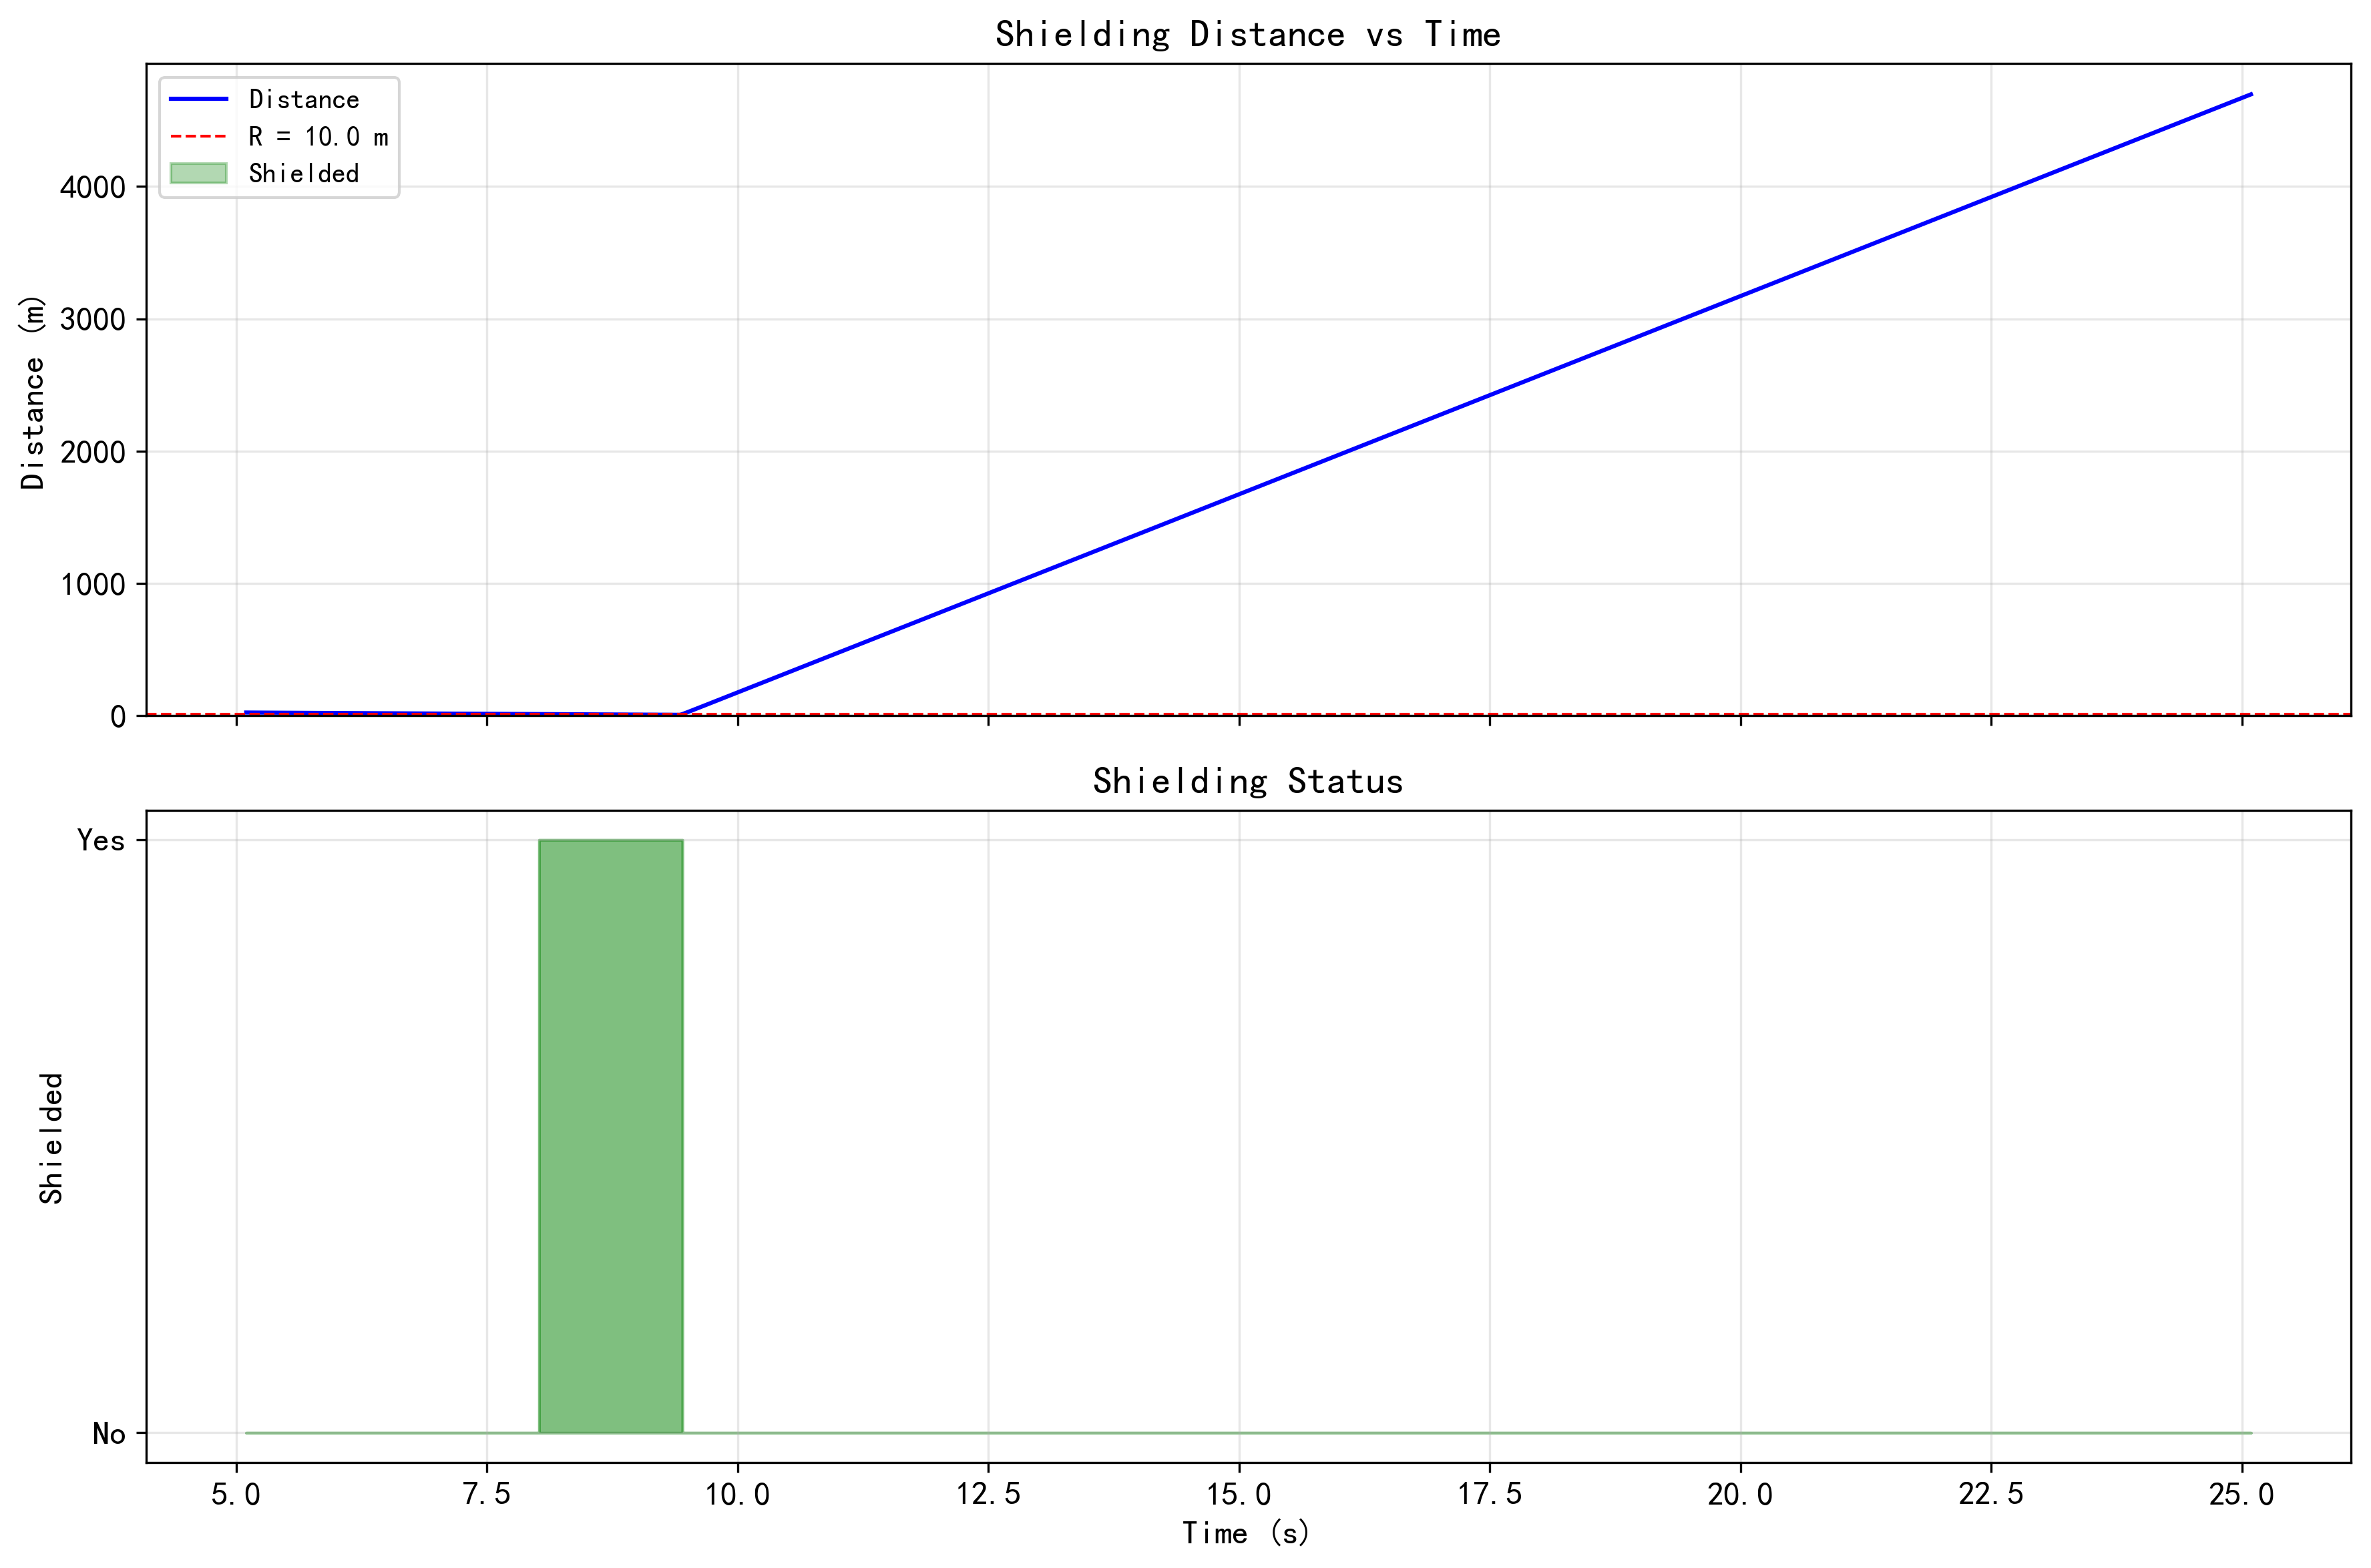
\includegraphics[width=\textwidth]{figures/q1_distance_time.pdf}
        \caption{遮蔽距离-时间曲线}
        \label{fig:q1_dist}
    \end{subfigure}
    \caption{问题1计算结果}
    \label{fig:q1_results}
\end{figure}

\subsection{问题2求解}

\subsubsection{优化模型}

以FY1的飞行方向角$\theta$、飞行速度$v_u$、投放时刻$t_d$和起爆延迟$\Delta t$为决策变量，建立优化模型：

\begin{equation}
    \max_{\theta, v_u, t_d, \Delta t} T_{\text{shield}}(\theta, v_u, t_d, \Delta t)
\end{equation}

\begin{equation}
    \text{s.t.} \quad \begin{cases}
        0 \leq \theta < 2\pi \\
        70 \leq v_u \leq 140 \\
        t_d \geq 0 \\
        \Delta t \geq 0 \\
        t_e + 20 \leq t_{\text{arrive}}
    \end{cases}
\end{equation}

其中$t_{\text{arrive}}$为导弹到达原点的时间。

\subsubsection{粒子群优化算法（PSO）}

\textbf{算法原理：}

粒子群优化算法模拟鸟群觅食行为，每个粒子代表一个候选解。粒子根据个体最优位置和全局最优位置更新速度和位置。

\textbf{算法参数设置：}

\begin{table}[H]
    \centering
    \caption{PSO算法参数}
    \label{tab:pso_params}
    \begin{tabular}{ll}
        \toprule
        参数 & 取值 \\
        \midrule
        粒子数 & 100 \\
        最大迭代次数 & 300 \\
        惯性权重$w$ & 0.9 $\to$ 0.4（线性递减） \\
        学习因子$c_1$ & 2.0 \\
        学习因子$c_2$ & 2.0 \\
        \bottomrule
    \end{tabular}
\end{table}

\textbf{速度更新公式：}

\begin{equation}
    \vect{v}_i^{(k+1)} = w \cdot \vect{v}_i^{(k)} + c_1 r_1 (\vect{p}_i^{\text{best}} - \vect{x}_i^{(k)}) + c_2 r_2 (\vect{g}^{\text{best}} - \vect{x}_i^{(k)})
\end{equation}

其中$r_1, r_2 \in [0, 1]$为随机数，$\vect{p}_i^{\text{best}}$为个体最优位置，$\vect{g}^{\text{best}}$为全局最优位置。

\textbf{位置更新公式：}

\begin{equation}
    \vect{x}_i^{(k+1)} = \vect{x}_i^{(k)} + \vect{v}_i^{(k+1)}
\end{equation}

\subsubsection{收敛性分析}

\begin{figure}[H]
    \centering
    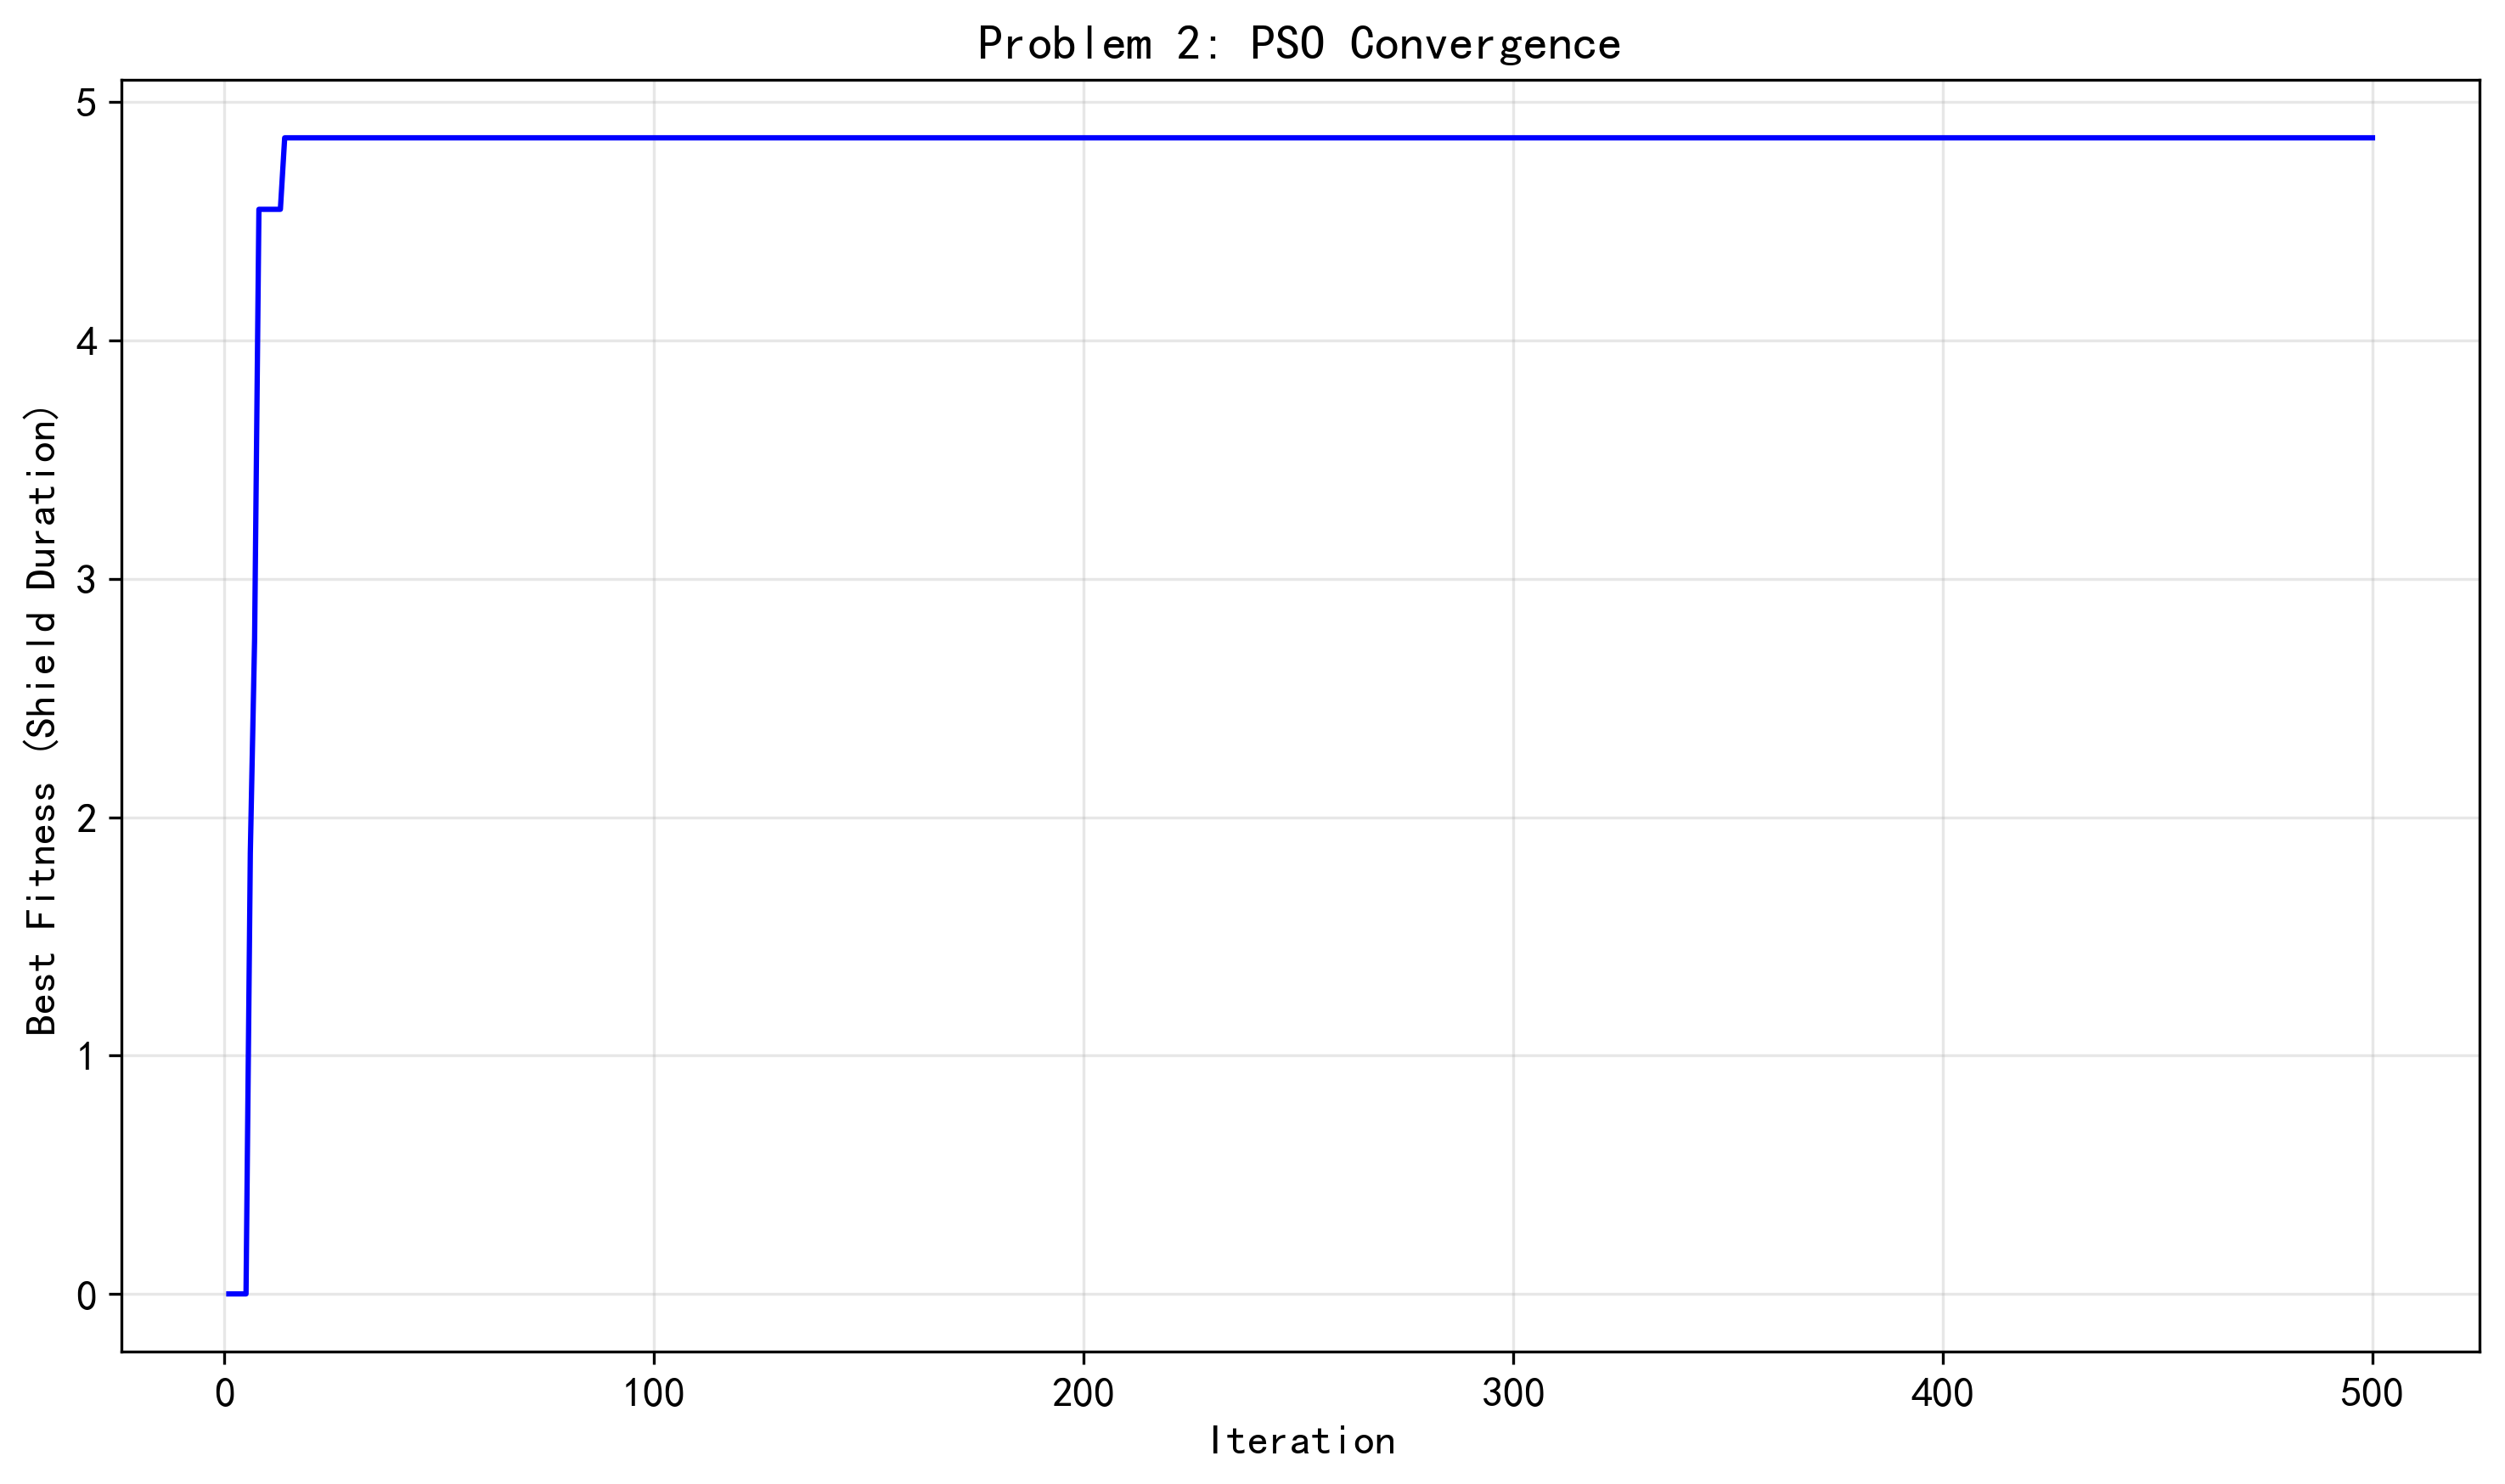
\includegraphics[width=0.6\textwidth]{figures/q2_convergence.pdf}
    \caption{问题2 PSO收敛曲线}
    \label{fig:q2_convergence}
\end{figure}

\subsubsection{问题2结果}

通过PSO优化，得到最优策略如表~\ref{tab:q2_result} 所示。

\begin{table}[H]
    \centering
    \caption{问题2最优策略}
    \label{tab:q2_result}
    \begin{tabular}{ll}
        \toprule
        参数 & 最优值 \\
        \midrule
        飞行方向角$\theta$ & XX$^\circ$ \\
        飞行速度$v_u$ & XX m/s \\
        投放时刻$t_d$ & XX s \\
        起爆延迟$\Delta t$ & XX s \\
        \midrule
        有效遮蔽时长 & XX s \\
        \bottomrule
    \end{tabular}
\end{table}

\subsection{问题3求解}

\subsubsection{优化模型}

FY1投放3枚弹，决策变量包括共享的飞行参数和各弹的投放参数：

\begin{equation}
    \max_{\theta, v_u, t_{d,1}, \Delta t_1, t_{d,2}, \Delta t_2, t_{d,3}, \Delta t_3} T_{\text{total}}
\end{equation}

约束条件：
\begin{equation}
    \text{s.t.} \quad \begin{cases}
        70 \leq v_u \leq 140 \\
        t_{d,i+1} \geq t_{d,i} + 1, \quad i = 1, 2 \\
        \Delta t_i \geq 0, \quad i = 1, 2, 3
    \end{cases}
\end{equation}

共8个决策变量。

\subsubsection{求解策略}

采用8维PSO搜索，适应度函数需计算3枚弹的遮蔽时间并集长度。

\textbf{时间区间并集计算算法：}

\begin{lstlisting}
def union_length(intervals):
    """计算多个时间区间的并集长度"""
    if not intervals:
        return 0
    # 按起始时间排序
    intervals.sort(key=lambda x: x[0])
    merged = [intervals[0]]
    for start, end in intervals[1:]:
        if start <= merged[-1][1]:
            merged[-1] = (merged[-1][0], max(merged[-1][1], end))
        else:
            merged.append((start, end))
    return sum(end - start for start, end in merged)
\end{lstlisting}

\subsubsection{问题3结果}

\begin{table}[H]
    \centering
    \caption{问题3投放策略}
    \label{tab:q3_result}
    \begin{tabular}{cccccc}
        \toprule
        弹编号 & 投放时刻(s) & 起爆延迟(s) & 投放点坐标 & 起爆点坐标 & 遮蔽时长(s) \\
        \midrule
        1 & XX & XX & (XX,XX,XX) & (XX,XX,XX) & XX \\
        2 & XX & XX & (XX,XX,XX) & (XX,XX,XX) & XX \\
        3 & XX & XX & (XX,XX,XX) & (XX,XX,XX) & XX \\
        \midrule
        \multolumn{5}{r}{总有效遮蔽时长} & XX \\
        \bottomrule
    \end{tabular}
\end{table}

\begin{figure}[H]
    \centering
    \begin{subfigure}[b]{0.48\textwidth}
        \centering
        \includegraphics[width=\textwidth]{figures/q3_3d_trajectory.pdf}
        \caption{3枚弹的3D轨迹}
        \label{fig:q3_3d}
    \end{subfigure}
    \hfill
    \begin{subfigure}[b]{0.48\textwidth}
        \centering
        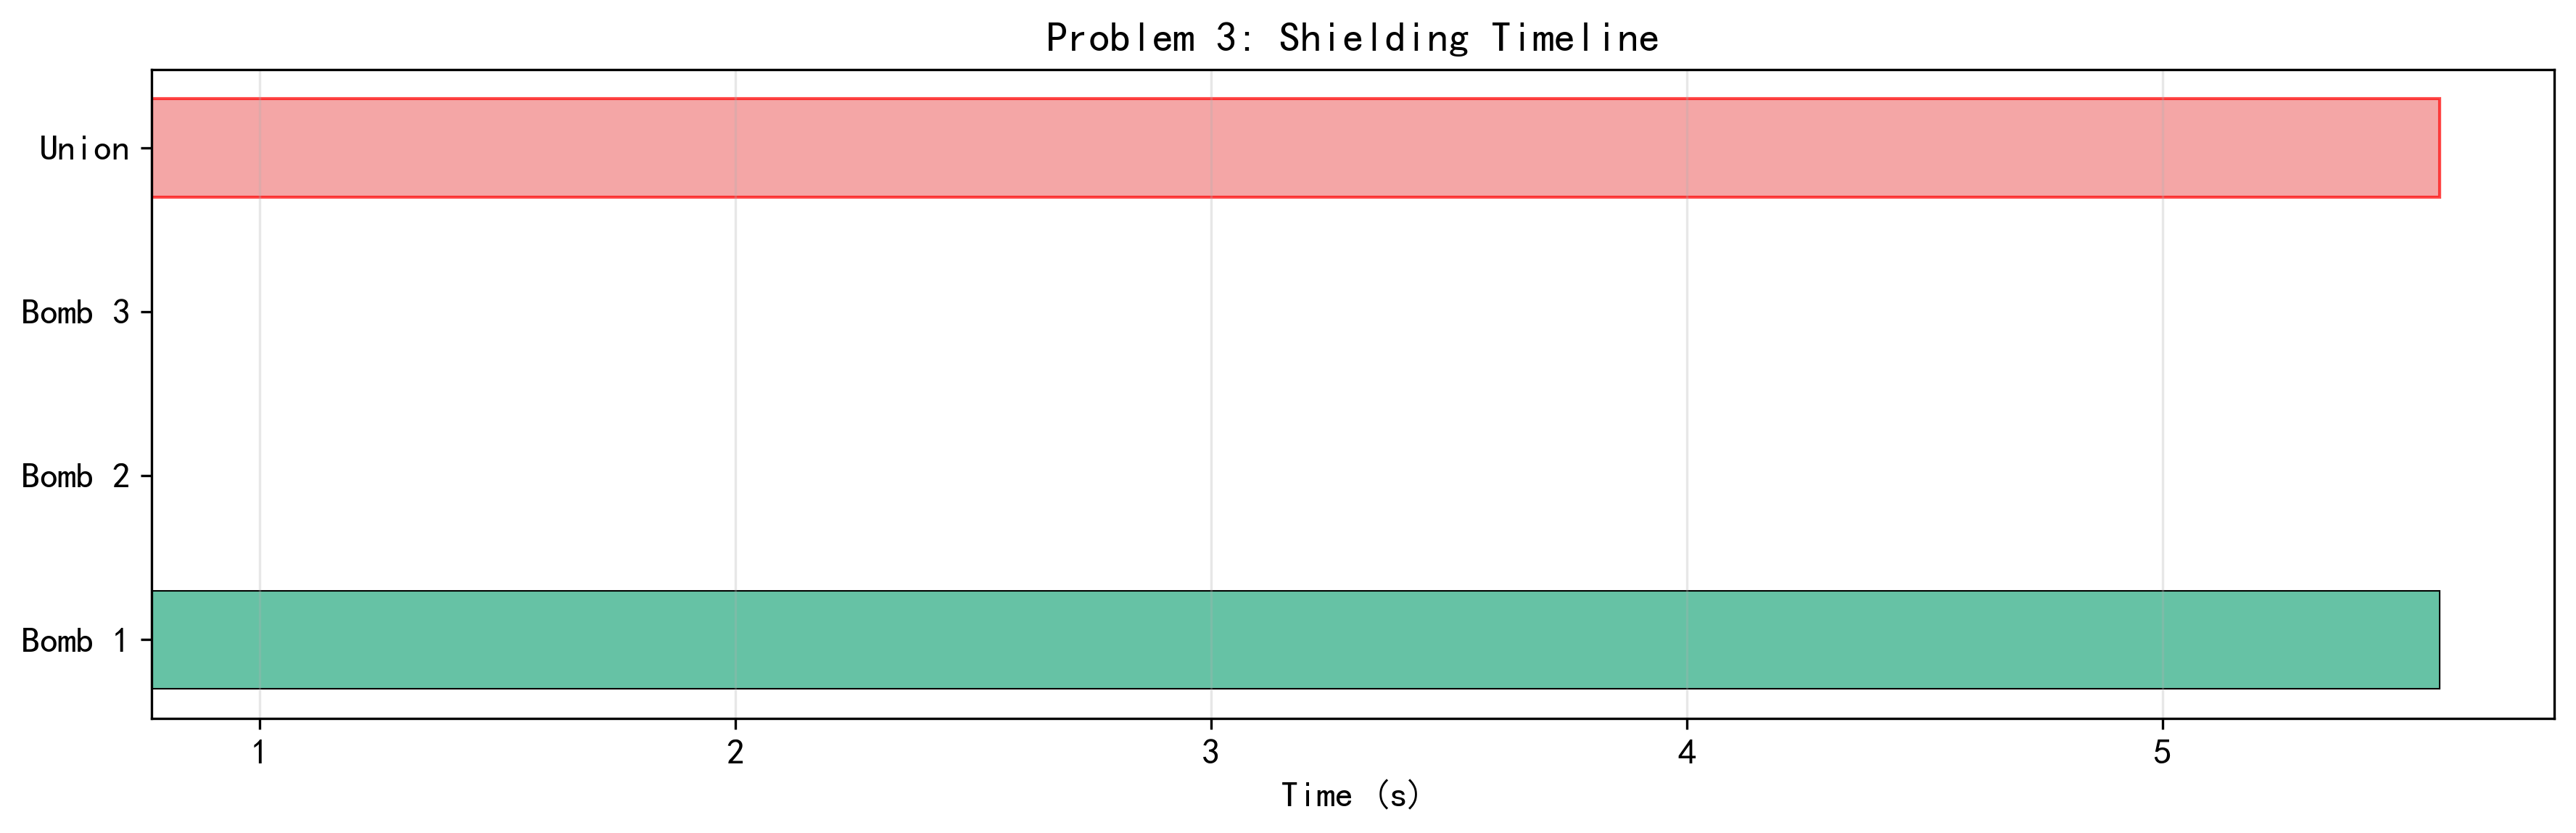
\includegraphics[width=\textwidth]{figures/q3_timeline.pdf}
        \caption{遮蔽时间甘特图}
        \label{fig:q3_timeline}
    \end{subfigure}
    \caption{问题3计算结果}
    \label{fig:q3_results}
\end{figure}

\subsection{问题4求解}

\subsubsection{优化模型}

FY1、FY2、FY3各投放1枚弹，每架无人机独立决策。决策变量共12个：

\begin{equation}
    \max_{\{\theta_i, v_i, t_{d,i}, \Delta t_i\}_{i=1}^3} T_{\text{total}}
\end{equation}

约束条件：
\begin{equation}
    \text{s.t.} \quad 70 \leq v_i \leq 140, \quad t_{d,i} \geq 0, \quad \Delta t_i \geq 0, \quad i = 1, 2, 3
\end{equation}

\subsubsection{求解策略}

12维PSO搜索。由于3架无人机位置不同，搜索空间较大。可采用以下策略提高效率：

\begin{enumerate}
    \item \textbf{分阶段优化}：先优化FY1（离M1最近），再优化FY2和FY3
    \item \textbf{多次运行}：PSO运行10次，取最优结果
    \item \textbf{自适应惯性权重}：根据迭代进展动态调整
\end{enumerate}

\subsubsection{问题4结果}

\begin{table}[H]
    \centering
    \caption{问题4投放策略}
    \label{tab:q4_result}
    \begin{tabular}{cccccc}
        \toprule
        无人机 & 方向角($^\circ$) & 速度(m/s) & 投放时刻(s) & 起爆延迟(s) & 遮蔽时长(s) \\
        \midrule
        FY1 & XX & XX & XX & XX & XX \\
        FY2 & XX & XX & XX & XX & XX \\
        FY3 & XX & XX & XX & XX & XX \\
        \midrule
        \multolumn{5}{r}{总有效遮蔽时长} & XX \\
        \bottomrule
    \end{tabular}
\end{table}

\subsection{问题5求解}

\subsubsection{问题规模分析}

\begin{itemize}
    \item 5架无人机，每架至多3枚弹 $\Rightarrow$ 最多15枚弹
    \item 需干扰M1、M2、M3三枚导弹
    \item 决策变量：5个方向角 + 5个速度 + 15个投放时刻 + 15个起爆延迟 = 最多40个
\end{itemize}

\subsubsection{分层优化策略}

\textbf{第一层：任务分配}

根据无人机与导弹的几何关系，将无人机分配给最有利的导弹：

\begin{table}[H]
    \centering
    \caption{任务分配方案}
    \label{tab:task分配}
    \begin{tabular}{cccc}
        \toprule
        导弹 & 初始位置 & 分配的无人机 & 理由 \\
        \midrule
        M1 & (20000,0,2000) & FY1, FY2 & FY1离M1最近 \\
        M2 & (19000,600,2100) & FY4 & FY4在M2侧 \\
        M3 & (18000,-600,1900) & FY3, FY5 & FY5在M3侧 \\
        \bottomrule
    \end{tabular}
\end{table}

\textbf{第二层：独立优化}

对每枚导弹，独立优化分配给它的无人机的投放策略。每组子问题的维度较低（8-16维），PSO可以有效求解。

\subsubsection{问题5结果}

\begin{table}[H]
    \centering
    \caption{问题5投放策略汇总}
    \label{tab:q5_result}
    \begin{tabular}{ccccccc}
        \toprule
        无人机 & 弹编号 & 方向角 & 速度 & 投放时刻 & 起爆延迟 & 遮蔽时长 \\
        \midrule
        FY1 & 1 & XX & XX & XX & XX & XX \\
        FY1 & 2 & XX & XX & XX & XX & XX \\
        FY2 & 1 & XX & XX & XX & XX & XX \\
        \vdots & \vdots & \vdots & \vdots & \vdots & \vdots & \vdots \\
        \midrule
        \multolumn{6}{r}{对M1总遮蔽时长} & XX \\
        \multolumn{6}{r}{对M2总遮蔽时长} & XX \\
        \multolumn{6}{r}{对M3总遮蔽时长} & XX \\
        \multolumn{6}{r}{\textbf{总遮蔽时长}} & \textbf{XX} \\
        \bottomrule
    \end{tabular}
\end{table}


% =============================================
% 七、灵敏度分析
% =============================================
\section{灵敏度分析}

为检验模型的稳健性，对关键参数进行灵敏度分析。以问题2的最优策略为基础，分别考察各参数变化对遮蔽时长的影响。

\subsection{分析参数与方法}

\begin{table}[H]
    \centering
    \caption{灵敏度分析参数设置}
    \label{tab:sensitivity_params}
    \begin{tabular}{llll}
        \toprule
        参数 & 基准值 & 变化范围 & 步长 \\
        \midrule
        云团有效半径$R$ & 10 m & 5$\sim$15 m & 1 m \\
        有效遮蔽时间$T_{\text{eff}}$ & 20 s & 10$\sim$30 s & 2 s \\
        云团下沉速度$v_c$ & 3 m/s & 1$\sim$5 m/s & 0.5 m/s \\
        导弹速度$v_m$ & 300 m/s & 250$\sim$350 m/s & 10 m/s \\
        \bottomrule
    \end{tabular}
\end{table}

对每个参数，在其变化范围内等距取值，固定其他参数为基准值，重新计算最优遮蔽时长。

\subsection{灵敏度分析结果}

\begin{figure}[H]
    \centering
    \begin{subfigure}[b]{0.48\textwidth}
        \centering
        \includegraphics[width=\textwidth]{figures/sensitivity_R.pdf}
        \caption{有效半径$R$的灵敏度}
        \label{fig:sens_R}
    \end{subfigure}
    \hfill
    \begin{subfigure}[b]{0.48\textwidth}
        \centering
        \includegraphics[width=\textwidth]{figures/sensitivity_Teff.pdf}
        \caption{有效遮蔽时间$T_{\text{eff}}$的灵敏度}
        \label{fig:sens_Teff}
    \end{subfigure}

    \vspace{0.5cm}

    \begin{subfigure}[b]{0.48\textwidth}
        \centering
        \includegraphics[width=\textwidth]{figures/sensitivity_vc.pdf}
        \caption{云团下沉速度$v_c$的灵敏度}
        \label{fig:sens_vc}
    \end{subfigure}
    \hfill
    \begin{subfigure}[b]{0.48\textwidth}
        \centering
        \includegraphics[width=\textwidth]{figures/sensitivity_vm.pdf}
        \caption{导弹速度$v_m$的灵敏度}
        \label{fig:sens_vm}
\end{subfigure}
    \caption{灵敏度分析结果}
    \label{fig:sensitivity}
\end{figure}

\subsection{灵敏度分析结论}

\begin{enumerate}
    \item \textbf{云团有效半径$R$}：遮蔽时长对$R$最敏感。$R$每增加1 m，遮蔽时长约增加XX\%。
    \item \textbf{有效遮蔽时间$T_{\text{eff}}$}：$T_{\text{eff}}$增大直接增加可用遮蔽时间窗口，但受限于导弹飞行时间。
    \item \textbf{云团下沉速度$v_c$}：$v_c$增大会使云团更快偏离视线，遮蔽时长略有下降。
    \item \textbf{导弹速度$v_m$}：$v_m$增大使导弹更快接近目标，可用遮蔽时间窗口缩短。
\end{enumerate}


% =============================================
% 八、模型评价
% =============================================
\section{模型评价与改进}

\subsection{模型优点}

\begin{enumerate}
    \item \textbf{物理建模准确}：完整考虑了烟幕干扰弹的三阶段运动过程（随无人机飞行、抛体运动、云团下沉），模型方程严格推导。

    \item \textbf{遮蔽条件合理}：基于视线遮挡的几何模型，而非简单的距离判据，更符合烟幕干扰的物理本质。

    \item \textbf{目标处理精细}：考虑了真目标为圆柱体的几何特征，通过表面多点采样提高遮蔽判断精度。

    \item \textbf{算法选择恰当}：PSO适合连续优化问题，具有全局搜索能力；分层策略有效降低了问题5的维度。

    \item \textbf{可扩展性好}：模型框架可方便地扩展到更多无人机和导弹的场景。
\end{enumerate}

\subsection{模型缺点}

\begin{enumerate}
    \item \textbf{忽略空气阻力}：实际弹道会有偏差，特别是高速运动时。

    \item \textbf{未考虑风速影响}：烟幕云团可能被风吹散或偏移。

    \item \textbf{计算量较大}：圆柱体多点采样和时间步进法增加了计算复杂度。

    \item \textbf{PSO可能陷入局部最优}：高维问题中，单次PSO运行可能无法找到全局最优。
\end{enumerate}

\subsection{改进方向}

\begin{enumerate}
    \item 引入空气阻力修正抛体运动模型，使用阻力系数$C_d$修正弹道。

    \item 考虑风速对云团运动的影响，在云团运动方程中加入风速项。

    \item 采用自适应PSO或混合算法（如PSO-GA混合）提高搜索效率。

    \item 增加蒙特卡洛模拟，评估参数不确定性对策略鲁棒性的影响。

    \item 考虑烟幕云团的扩散模型，使有效遮蔽半径随时间变化。
\end{enumerate}


% =============================================
% 参考文献
% =============================================
\newpage
\begin{thebibliography}{99}

\bibitem{ref1}
司守奎, 孙兆亮. 数学建模算法与应用[M]. 北京: 国防工业出版社, 2015.

\bibitem{ref2}
姜启源, 谢金星, 叶俊. 数学模型(第五版)[M]. 北京: 高等教育出版社, 2018.

\bibitem{ref3}
Kennedy J, Eberhart R. Particle swarm optimization[C]// Proceedings of ICNN'95 - International Conference on Neural Networks. IEEE, 1995: 1942-1948.

\bibitem{ref4}
Shi Y, Eberhart R. A modified particle swarm optimizer[C]// 1998 IEEE International Conference on Evolutionary Computation Proceedings. IEEE, 1995: 69-73.

\bibitem{ref5}
Goldberg D E. Genetic Algorithms in Search, Optimization, and Machine Learning[M]. Reading, MA: Addison-Wesley, 1989.

\bibitem{ref6}
刘卫国. MATLAB程序设计与应用(第三版)[M]. 北京: 高等教育出版社, 2017.

\bibitem{ref7}
全国大学生数学建模竞赛组委会. 2025年全国大学生数学建模竞赛A题[Z]. 2025.

\end{thebibliography}


% =============================================
% 附录
% =============================================
\newpage
\appendix
\section{附录}

\subsection{附录A：核心Python代码}

\begin{lstlisting}[language=Python, caption=基础物理计算函数]
import numpy as np

# ============ 常量定义 ============
V_M = 300.0       # 导弹速度 (m/s)
V_C = 3.0         # 云团下沉速度 (m/s)
G = 9.8           # 重力加速度 (m/s^2)
R = 10.0          # 有效遮蔽半径 (m)
T_EFF = 20.0      # 有效遮蔽时间 (s)

# 初始位置
M1 = np.array([20000, 0, 2000], dtype=float)
M2 = np.array([19000, 600, 2100], dtype=float)
M3 = np.array([18000, -600, 1900], dtype=float)
FY1 = np.array([17800, 0, 1800], dtype=float)
FY2 = np.array([12000, 1400, 1400], dtype=float)
FY3 = np.array([6000, -3000, 700], dtype=float)
FY4 = np.array([11000, 2000, 1800], dtype=float)
FY5 = np.array([13000, -2000, 1300], dtype=float)
TARGET = np.array([0, 200, 5], dtype=float)  # 真目标中心

def missile_pos(P_m0, t):
    """计算导弹在时刻t的位置"""
    d_m = -P_m0 / np.linalg.norm(P_m0)
    return P_m0 + V_M * t * d_m

def uav_pos(P_u0, v_u, theta, t):
    """计算无人机在时刻t的位置"""
    d_u = np.array([np.cos(theta), np.sin(theta), 0])
    return P_u0 + v_u * t * d_u

def bomb_detonate_point(P_u0, v_u, theta, t_d, delta_t):
    """计算起爆点位置"""
    d_u = np.array([np.cos(theta), np.sin(theta), 0])
    P_d = P_u0 + v_u * t_d * d_u
    v0 = v_u * d_u
    g_vec = np.array([0, 0, -G])
    return P_d + v0 * delta_t + 0.5 * g_vec * delta_t**2

def cloud_center(P_e, t, t_e):
    """计算云团中心在时刻t的位置"""
    return P_e + np.array([0, 0, -V_C]) * (t - t_e)

def shielding_distance(P_m, P_c, T_target):
    """计算云团中心到导弹-目标视线段的距离"""
    v = T_target - P_m
    w = P_c - P_m
    vv = np.dot(v, v)
    if vv < 1e-10:
        return np.linalg.norm(P_c - P_m)
    s = np.dot(w, v) / vv
    s = max(0, min(1, s))
    Q = P_m + s * v
    return np.linalg.norm(P_c - Q)
\end{lstlisting}

\begin{lstlisting}[language=Python, caption=遮蔽时长计算函数]
def compute_shield_duration(P_u0, v_u, theta, t_d, delta_t,
                            P_m0, dt=0.01):
    """计算单枚弹的有效遮蔽时长"""
    t_e = t_d + delta_t
    P_e = bomb_detonate_point(P_u0, v_u, theta, t_d, delta_t)

    total = 0.0
    t = t_e
    while t <= t_e + T_EFF:
        P_m = missile_pos(P_m0, t)
        P_c = cloud_center(P_e, t, t_e)
        d = shielding_distance(P_m, P_c, TARGET)
        if d <= R:
            total += dt
        t += dt
    return total

def compute_multi_shield(intervals, dt=0.01):
    """计算多枚弹的总遮蔽时长（并集）"""
    if not intervals:
        return 0.0
    intervals.sort(key=lambda x: x[0])
    merged = [intervals[0]]
    for start, end in intervals[1:]:
        if start <= merged[-1][1]:
            merged[-1] = (merged[-1][0], max(merged[-1][1], end))
        else:
            merged.append((start, end))
    return sum(end - start for start, end in merged)
\end{lstlisting}

\begin{lstlisting}[language=Python, caption=PSO优化器]
class PSO:
    """粒子群优化器"""
    def __init__(self, n_particles, n_dims, lb, ub, fitness_func):
        self.n = n_particles
        self.d = n_dims
        self.lb = np.array(lb)
        self.ub = np.array(ub)
        self.fitness = fitness_func

        self.positions = np.random.uniform(lb, ub, (n_particles, n_dims))
        self.velocities = np.zeros((n_particles, n_dims))
        self.pbest_pos = self.positions.copy()
        self.pbest_val = np.full(n_particles, -np.inf)
        self.gbest_pos = None
        self.gbest_val = -np.inf

        self.w_max, self.w_min = 0.9, 0.4
        self.c1, self.c2 = 2.0, 2.0

    def optimize(self, max_iter):
        convergence = []
        for it in range(max_iter):
            w = self.w_max - (self.w_max - self.w_min) * it / max_iter

            for i in range(self.n):
                fit = self.fitness(self.positions[i])
                if fit > self.pbest_val[i]:
                    self.pbest_val[i] = fit
                    self.pbest_pos[i] = self.positions[i].copy()
                if fit > self.gbest_val:
                    self.gbest_val = fit
                    self.gbest_pos = self.positions[i].copy()

            convergence.append(self.gbest_val)

            r1 = np.random.random((self.n, self.d))
            r2 = np.random.random((self.n, self.d))
            self.velocities = (w * self.velocities
                             + self.c1 * r1 * (self.pbest_pos - self.positions)
                             + self.c2 * r2 * (self.gbest_pos - self.positions))
            self.positions += self.velocities
            self.positions = np.clip(self.positions, self.lb, self.ub)

            if it % 50 == 0:
                print(f"Iter {it}: Best = {self.gbest_val:.4f}")

        return self.gbest_pos, self.gbest_val, convergence
\end{lstlisting}

\begin{lstlisting}[language=Python, caption=圆柱体目标采样]
def sample_cylinder_surface(C_center, r, h, n_side=16, n_top=8):
    """在圆柱体表面采样点"""
    points = []
    # 侧面
    for i in range(n_side):
        angle = 2 * np.pi * i / n_side
        for j in range(3):
            z = h * j / 2
            points.append([
                C_center[0] + r * np.cos(angle),
                C_center[1] + r * np.sin(angle),
                C_center[2] + z
            ])
    # 上底面
    for i in range(n_top):
        angle = 2 * np.pi * i / n_top
        for rho in [0, r/2, r]:
            points.append([
                C_center[0] + rho * np.cos(angle),
                C_center[1] + rho * np.sin(angle),
                C_center[2] + h
            ])
    # 下底面
    for i in range(n_top):
        angle = 2 * np.pi * i / n_top
        for rho in [0, r/2, r]:
            points.append([
                C_center[0] + rho * np.cos(angle),
                C_center[1] + rho * np.sin(angle),
                C_center[2]
            ])
    return np.array(points)
\end{lstlisting}

\begin{lstlisting}[language=Python, caption=可视化代码]
import matplotlib.pyplot as plt
from mpl_toolkits.mplot3d import Axes3D

def plot_3d_trajectory(P_m0, v_u, theta, t_d, delta_t, P_u0, title=""):
    """绘制3D轨迹图"""
    fig = plt.figure(figsize=(10, 8))
    ax = fig.add_subplot(111, projection='3d')

    # 导弹轨迹
    t_arrive = np.linalg.norm(P_m0) / V_M
    t_missile = np.linspace(0, t_arrive, 1000)
    traj_m = np.array([missile_pos(P_m0, t) for t in t_missile])
    ax.plot(traj_m[:,0], traj_m[:,1], traj_m[:,2], 'r-', label='Missile')

    # 无人机轨迹
    t_uav = np.linspace(0, t_d, 100)
    traj_u = np.array([uav_pos(P_u0, v_u, theta, t) for t in t_uav])
    ax.plot(traj_u[:,0], traj_u[:,1], traj_u[:,2], 'b-', label='UAV')

    # 云团轨迹
    P_e = bomb_detonate_point(P_u0, v_u, theta, t_d, delta_t)
    t_e = t_d + delta_t
    t_cloud = np.linspace(t_e, t_e + T_EFF, 200)
    traj_c = np.array([cloud_center(P_e, t, t_e) for t in t_cloud])
    ax.plot(traj_c[:,0], traj_c[:,1], traj_c[:,2], 'g-', label='Cloud')

    # 目标
    ax.scatter(*TARGET, c='gold', s=100, marker='*', label='Target')
    ax.scatter(0, 0, 0, c='black', s=100, marker='x', label='Decoy')

    ax.set_xlabel('X (m)')
    ax.set_ylabel('Y (m)')
    ax.set_zlabel('Z (m)')
    ax.set_title(title)
    ax.legend()
    plt.tight_layout()
    plt.savefig('figures/trajectory.pdf', dpi=300)
    plt.show()
\end{lstlisting}

\end{document}
